\chapter{Basics of Groups}
With a basic intuition of the definition of groups, we look at the basic properties satisfied by groups and introduce two simple types of groups.

\section{Basic Examples of Groups}
Recall that a group satisfies four axioms.
\begin{enumerate}
    \item \textbf{Closure}: For all elements $a$ and $b$ in $G$, $a \ast b$ is also in $G$.
    \item \textbf{Associativity}: For all elements $a, b$, and $c$ in $G$, we have $a \ast (b \ast c) = (a \ast b) \ast c$.
    \item \textbf{Identity}: There exists an element $e$ in $G$, called the identity element\index{group!identity}, such that, for any element $x$ in $G$, we have $e \ast x = x \ast e = x$.
    \item \textbf{Inverse}: For every element $x$ in $G$, there exists an element $x^{-1}$ in $G$ such that $x \ast x^{-1} = x^{-1} \ast x = e$.
\end{enumerate}

Recall also we write $a \ast b$ as $ab$, and denote the group $(G, \ast)$ by $G$ only.

\begin{remark}
    If the group operation is additive\index{group!additive}, we write $a + b$ instead of $ab$.
\end{remark}

Let's look at some examples of groups.

\newpage

\begin{example}
    Let $\mathbb{Z}$ be the set of integers and let $+$ denote regular addition. Then $(\mathbb{Z}, +)$ forms a group.
    \begin{enumerate}
        \item \textbf{Closure}: For all integers $a$ and $b$, we know $a + b$ is an integer.
        \item \textbf{Associativity}: We know $a + (b + c) = (a + b) + c$.
        \item \textbf{Identity}: The identity is 0, since $0 + x = x + 0 = x$.
        \item \textbf{Inverse}: The inverse of the integer $x$ is $-x$, since $x + (-x) = (-x) + x = 0$.
    \end{enumerate}
\end{example}

An important thing to note about addition is that it is \textit{commutative}: $a + b = b + a$. A group with a commutative operation is called a \textbf{commutative group}\index{group!commutative}. However, it is more often called an \textbf{abelian group}\index{group!abelian}, named after Norwegian mathematician Niels Henrik Abel.

We now look at the notion of $\mathbb{Z}_n$.
\begin{definition}
    The set $\mathbb{Z}_n = \{0, 1, 2, \dots, n-1\}$ where $n$ is a non-negative integer.
\end{definition}
\begin{proposition}
    The set $\mathbb{Z}_n$ with the operation $\oplus_n$ forms a group, where $\oplus_n$ is addition modulo $n$. That is, $a \oplus_n b = (a + b) \mod{n}$.
\end{proposition}
\begin{proof}
    We prove this by showing the group axioms hold.
    \begin{enumerate}
        \item \textbf{Closure}: For $a$ and $b$ in $\mathbb{Z}_n$, $a \oplus_n b = (a + b) \mod{n}$ is a integer between 0 and $n - 1$. Thus $a \oplus b$ is inside $\mathbb{Z}_n$.
        \item \textbf{Associativity}: For $a$, $b$, and $c$ in $\mathbb{Z}_n$, since addition is associative, thus $a \oplus_n (b \oplus_n c) = (a + (b + c)) \mod{n} = ((a + b) + c) \mod{n} = (a \oplus_n b) \oplus_n c$.
        \item \textbf{Identity}: The identity is $0$ since for every $x$ in $\mathbb{Z}_n$, $0 \oplus_n x = (0 + x) \mod{n} = (x + 0) \mod{n} = x \oplus_n 0 = x$.
        \item \textbf{Inverse}:
        \begin{itemize}
            \item $0$ is its own inverse since $0 \oplus_n 0 = 0$ which is the identity.
            \item For any other integer $x$ in $\mathbb{Z}_n$, the inverse is $n - x$. Since $1 \leq x \leq n - 1$, thus $1 \leq n - x \leq n - 1$ so $n - x$ is indeed in $\mathbb{Z}_n$. Also, $x \oplus_n (n - x) = (x + (n - x)) \mod{n} = n \mod{n} = 0$ and $(n - x) \oplus_n x = ((n-x) + x)\mod{n} = n \mod{n} = 0$.
        \end{itemize}
    \end{enumerate}
    Since the four group axioms are satisfied, this is a group.
\end{proof}
\begin{remark}
    Some sources (e.g. \cite{clark_1984, humphreys_1996}) define $\mathbb{Z}_n$ as a set of congruence classes modulo $n$, i.e. $\mathbb{Z}/n\mathbb{Z}$. We will show that these two definitions are equivalent in a future chapter.
\end{remark}

One could use a \textbf{Cayley table}\index{cayley table} (or \textbf{group table}\index{group table}) to show that a structure is a group.
\begin{example}
    We show that $(\mathbb{Z}_6, \oplus_6)$ is a group by drawing the Cayley table of that structure.
    \begin{table}[h]
        \centering
        \begin{tabular}{|l|l|l|l|l|l|l|}
        \hline
        $\boldsymbol{\oplus_6}$ & $\boldsymbol{0}$ & $\boldsymbol{1}$ & $\boldsymbol{2}$ & $\boldsymbol{3}$ & $\boldsymbol{4}$ & $\boldsymbol{5}$ \\ \hline
        $\boldsymbol{0}$          & 0          & 1          & 2          & 3          & 4          & 5          \\ \hline
        $\boldsymbol{1}$          & 1          & 2          & 3          & 4          & 5          & 0          \\ \hline
        $\boldsymbol{2}$          & 2          & 3          & 4          & 5          & 0          & 1          \\ \hline
        $\boldsymbol{3}$          & 3          & 4          & 5          & 0          & 1          & 2          \\ \hline
        $\boldsymbol{4}$          & 4          & 5          & 0          & 1          & 2          & 3          \\ \hline
        $\boldsymbol{5}$          & 5          & 0          & 1          & 2          & 3          & 4          \\ \hline
        \end{tabular}
    \end{table}

    \newpage

    One observes from the above table that
    \begin{enumerate}
        \item for all $x$ and $y$ in $\mathbb{Z}_6$, $x \oplus_6 y$ is in $\mathbb{Z}_6$;
        \item for all $x, y$, and $z$ in $\mathbb{Z}_6$, $x \oplus_6 (y \oplus_6 z) = (x \oplus_6 y) \oplus_6 z$;
        \item 0 is the identity since adding anything to it returns the original number; and
        \item every row has an integer that, when added, gives 0.
    \end{enumerate}
    Thus $(\mathbb{Z}_6, \oplus_6)$ is a group.
\end{example}

It should be noted that, in this book, we use the convention of reading the \textbf{row before the column} in a group table. However, since $(\mathbb{Z}_6, \oplus_6)$ is an abelian group, the order does not matter. We will look at Cayley tables of non-abelian groups later.

\begin{exercise}
    Let $\otimes_n$ denote multiplication modulo $n$, i.e. $a \otimes_n b = (a \times b) \mod{n}$. By using a Cayley table, show that $(\mathbb{Z}_6, \otimes_6)$ does \textbf{not} form a group.
\end{exercise}

\section{General Properties of Groups}
Before we get into the general properties of groups, we introduce notation for the repeated application of $\ast$ on a single element $x$ in the group $G$.
\[
    x^n =
    \begin{cases}
        \underbrace{x\ast x\ast \cdots \ast x}_{n \text{ copies of } x} & \text{ if } n > 0\\
        e & \text{ if } n=0 \\
        \underbrace{x^{-1}\ast x^{-1}\ast \cdots \ast x^{-1}}_{|n| \text{ copies of } x^{-1}} & \text{ if } n<0
    \end{cases}
\]
In the case of an additive group operation, $x^n$ is written as $nx$, where $n$ is an integer.

Note that some laws of exponents apply to the above operation.
\begin{itemize}
    \item $\left(x^{-1}\right)^m = \left(x^m\right)^{-1}$
    \item $x^{m+n} = x^m \ast x^n$
    \item $\left(x^m\right)^n = x^{mn}$
\end{itemize}
Proof of these laws are left as an exercise for the reader.

We are now ready to prove some properties of groups.
\begin{proposition}
    The identity of a group $G$ is unique.
\end{proposition}
\begin{proof}
    Suppose $e_1$ and $e_2$ are identities of the group $G$. Then, for all $x$ in $G$, we have
    \[
        e_1x = xe_1 = x \text{ and } e_2x = xe_2 = x,
    \]
    since they are identities. Thus,
    \begin{align*}
        e_1 &= e_1e_2 & (e_2 \text{ is an identity, so } xe_2 = x)\\
        &= e_2 & (e_1 \text{ is an identity, so } xe_1 = x)
    \end{align*}
    Hence $e_1 = e_2$, meaning that the identity of a group is unique.
\end{proof}

\begin{proposition}
    $e^{-1} = e$
\end{proposition}
\begin{proof}
    Clearly $e = ee^{-1}$ since $xx^{-1} = e$ for all elements $x$ in $G$, including $x = e$. Thus, by left multiplying $e^{-1}$ on both sides, we see $e = e^{-1}$.
\end{proof}

\newpage

\begin{proposition}
    The inverse of an element $x$ of a group $G$ is unique.
\end{proposition}
\begin{proof}
    Suppose that $a$ and $b$ are inverses of $x$. Then by definition, $ax = xa = e \text{ and } bx = xb = e$. So,
    \begin{align*}
        a &= ae & (e \text{ is the identity})\\
        &= a(xb) & (b \text{ is an inverse, so } xb = e)\\
        &= (ax)b & (\text{associativity})\\
        &= eb & (a \text{ is an inverse, so } ax = e)\\
        &= b & (e \text{ is the identity})
    \end{align*}
    Therefore $a = b$. Thus the inverse of $x$ is unique.
\end{proof}

\begin{proposition}[Shoes and Socks]\index{Shoes and Socks}
    For all elements $a$ and $b$ in $G$, $(ab)^{-1} = b^{-1}a^{-1}$.
\end{proposition}
\begin{proof}
    Recall that if $g^{-1}$ is the inverse of $g$ then $gg^{-1} = g^{-1}g = e$. We will show that $(ab)(b^{-1}a^{-1}) = e$ and $(b^{-1}a^{-1})(ab) = e$.
    \begin{align*}
        (ab)(b^{-1}a^{-1}) &= a(bb^{-1})a^{-1} & (\text{associativity})\\
        &= a(e)a^{-1} & (bb^{-1} = e)\\
        &= aa^{-1} & (e \text{ is the identity})\\
        &= e & (aa^{-1} = e),
    \end{align*}
    and,
    \begin{align*}
        (b^{-1}a^{-1})(ab) &= b^{-1}(a^{-1}a)b & (\text{associativity})\\
        &= b^{-1}(e)b & (a^{-1}a = e)\\
        &= b^{-1}b & (e \text{ is the identity})\\
        &= e & ( b^{-1}b = e).
    \end{align*}
    Thus, $b^{-1}a^{-1}$ is the inverse of $ab$, so $(ab)^{-1} = b^{-1}a^{-1}$
\end{proof}

\begin{exercise}
Prove that for all $x$ in $G$, $\left(x^{-1}\right)^{-1} = x$.
\end{exercise}

We now prove an important property of groups: the \textbf{cancellation law}.
\begin{proposition}[Cancellation Law]\index{group!cancellation law}
    Let $g$, $x$, and $y$ be elements in the group $G$. Then
    \begin{enumerate}
        \item if $gx=gy$ then $x = y$; and
        \item if $xg=yg$ then $x = y$.
    \end{enumerate}
\end{proposition}
\begin{proof}
    We prove the two cases separately.
    \begin{enumerate}
        \item Suppose $gx = gy$. Then
        \begin{align*}
            &g^{-1}(gx) = g^{-1}(gy) & (\text{left multiply by } g^{-1})\\
            &(g^{-1}g)x = (g^{-1}g)y & (\text{associativity})\\
            &ex = ey & (g^{-1}g = e)\\
            &x = y & (e \text{ is the identity})
        \end{align*}
        \item Suppose $xg = yg$. Then
        \begin{align*}
            &(xg)g^{-1} = (yg)g^{-1} & (\text{right multiply by } g^{-1})\\
            &x(gg^{-1}) = y(gg^{-1}) & (\text{associativity})\\
            &xe = ye & (gg^{-1} = e)\\
            &x = y & (e \text{ is the identity})
        \end{align*}
    \end{enumerate}
    This completes the proof.
\end{proof}

\section{Order of a Group and Order of an Element}
We look at the notion of the \textit{order}\index{order} of a group and the order of an element of a group.

\begin{definition}
    Let $G$ be a group. The order of a group\index{order!group}, denoted by $|G|$, is the cardinality of the set $G$.
\end{definition}

If $|G| = n$ where $n$ is finite, we say that $G$ is a \textbf{finite group}. On the other hand, if $|G| = \infty$, then we say that $G$ is an \textbf{infinite group}.

\begin{example}
    The group $(\mathbb{Z}_4, \oplus_4)$ has order 4 since it has four elements: 0, 1, 2, and 3.
\end{example}

\begin{example}
    The group $(\mathbb{R}, +)$ is an infinite group since $\mathbb{R}$ has an uncountably infinite number of elements.
\end{example}

Let's now look at the order of an element.
\begin{definition}
    Let $g$ be an element of the group $G$. Then the order of $g$\index{order!element}, denoted by $|g|$, is the least positive integer $n$ such that $g^n = e$.
\end{definition}
Note that if $n$ is infinite, we say that the order of $g$ is infinite (or that $g$ has infinite order).

\begin{example}
    Consider the group $G = (\mathbb{Z}_4, \oplus_4)$ and its 4 elements 0, 1, 2, and 3.
    \begin{itemize}
        \item The element $0$ has order 1 since $0^1 = 0$, which is the identity. Thus $|0| = 1$ in $G$.
        \item The element $1$ has order 4 since $1 \oplus_4 1 \oplus_4 1 \oplus_4 1 = 0$ and no smaller $n$ than 4 exists. Thus $|1| = 4$ in $G$.
        \item The element $2$ has order 2 since $2 \oplus_4 2 = 0$ and no smaller $n$ than 2 exists. Thus $|2| = 2$ in $G$.
        \item The element $3$ has order 4 since $3 \oplus_4 3 \oplus_4 3 \oplus_4 3 = 0$ and no smaller $n$ than 4 exists. Thus $|3| = 4$ in $G$.
    \end{itemize}
\end{example}

We note a few things about the order of elements in a group.
\begin{itemize}
    \item The identity element always has order 1.
    \item A group in which every element has finite order is said to be \textbf{periodic}\index{group!periodic}.
    \item A finite group is always periodic because all elements in a finite group has finite order.
    \item The order of any element in a group divides the order of the group.
\end{itemize}
The last point is actually a consequence of Lagrange's Theorem (\myref{thrm-lagrange}). We will look into its proof in the next chapter.

\begin{exercise}
    Let $i$ be a number such that $i^2 = -1$. Let $\mathcal{S} = \{1, -1, i, -i\}$.
    \begin{partquestions}{\roman*}
        \item Find the identity of the group $(\mathcal{S}, \times)$ where $\times$ denotes regular multiplication.
        \item Find the orders of the elements of the above group.
    \end{partquestions}
\end{exercise}

\newpage

\section{Cyclic Groups}\index{cyclic group}
Now that we have gotten some basic terminology and properties of groups out of the way, let's introduce a very simple type of group: the cyclic groups.

\begin{definition}
    Let $G$ be a group and $g$ be in $G$. If
    \[
        G = \{g, g^2, g^3, \dots, g^n\}
    \]
    for some positive integer $n$, then $G$ is a \textbf{cyclic group of order $n$}\index{cyclic group!of order $n$} and has a \textbf{generator $g$}\index{cyclic group!generator}.
\end{definition}
Notationally, we write $G = \langle g \rangle$.

\begin{example}
    Let $i$ be the imaginary unit, i.e. $i^2 = -1$. Let $\mathcal{S} = \{1, -1, i, -i\}$. Notice the group $(\mathcal{S}, \times)$ is completely generated by the element $i$ since
    \[
    i^1 = i,\; i^2 = -1,\; i^3 = -i, \text{ and } i^4 = 1.
    \]
    Thus, $\mathcal{S} = \{i, i^2, i^3, i^4\} = \langle i \rangle$.
\end{example}

\begin{exercise}
    Using the set $\mathcal{S}$ from the above example, find the other generator of the group $(\mathcal{S}, \times)$.
\end{exercise}

It should be noted that not every element in a cyclic group is a generator, and that a cyclic group may have more than 1 generator.

Cyclic groups may also be of \textbf{infinite order}. Such cyclic groups are called \textbf{cyclic groups of infinite order} or \textbf{infinite cyclic groups}\index{cyclic group!infinite}.
\begin{example}
    The group $(\mathbb{Z}, +)$ is an infinite cyclic group with generators 1 and -1.
\end{example}

We now look at two results involving cyclic groups.

\begin{proposition}\label{prop-cyclic-group-is-abelian}
    Every cyclic group is abelian.
\end{proposition}
\begin{proof}
    Let $G$ be the cyclic group with a generator $g$. Suppose $x$ and $y$ are elements in $g$. Then $x = g^m$ and $y = g^n$ for some positive integers $m$ and $n$.

    Thus,
    \begin{align*}
        xy &= (g^m)(g^n)\\
        &= g^mg^n\\
        &= g^{m+n}\\
        &= g^{n+m} & (\text{+ is commutative})\\
        &= g^ng^m\\
        &= (g^n)(g^m)\\
        &= yx
    \end{align*}
    so $xy = yx$. Therefore $G$ is abelian.
\end{proof}

\begin{theorem}\label{thrm-cyclic-group-has-element-with-same-order}
    A finite group $G$ is cyclic if and only if there exists an element $g$ in $G$ with the same order as the group.
\end{theorem}
\begin{proof}
    We first prove the forward direction: suppose $G$ is cyclic and $|G| = n$. Then, by definition, there exists an element $g$ in $G$ such that
    \[
        G = \langle g \rangle = \{g^k \vert 1 \leq k \leq n, k \in \mathbb{Z}\},
    \]
    i.e. $g$ is a generator of $G$. We just need to show $|g| = n$.

    Suppose on the contrary there exists an integer $1 \leq m < n$ where $g^m = e$. Then $\langle g \rangle = \{g, g^2, \dots, g^m\}$. Thus $|\langle g \rangle| = m < n = |G|$. But by the hypothesis of the forward direction, $G = \langle g \rangle$ so $n = |G| = |\langle g \rangle| = m$. This is a contradiction, i.e. there does \textbf{not} exist an integer $1 \leq m < n$ where $g^m = e$. Therefore $g^n = e$, i.e. $|g| = n$.

    We now prove the reverse direction: suppose there exists an element $g$ in $G$ with order $n$.
    
    We claim that $g, g^2, \dots, g^n$ are all distinct. Suppose on the contrary that there exist integers $i$ and $j$ where $1 \leq i < j \leq n$ such that $g^i = g^j$. Then $g^i = g^ig^{j-i}$, which means $g^{j-i} = e$ by the cancellation law. Note that $1 \leq j - i < n$. Thus, since $g^{j-i} = e$, therefore $|g| = j - i < n$ which contradicts $|g| = n$. Hence, $g, g^2, \dots, g^n$ are all distinct. Therefore, $\langle g \rangle = \{g, g^2, \dots, g^n\}$ contain distinct elements of $G$. But there are only $n$ elements in $G$ and $\langle g \rangle$ contains $n$ distinct elements. Therefore, $G = \langle g \rangle$ which means that $G$ is cyclic with generator $g$.

    This completes the proof.
\end{proof}

There are more interesting properties of cyclic groups, but we will get to them when we develop more tools to explain and prove these properties.

\newpage

\section{Dihedral Groups}
We motivate the definition of the dihedral groups by discussing the symmetries of an equilateral triangle.

\begin{figure}[h]
    \centering
    \fbox{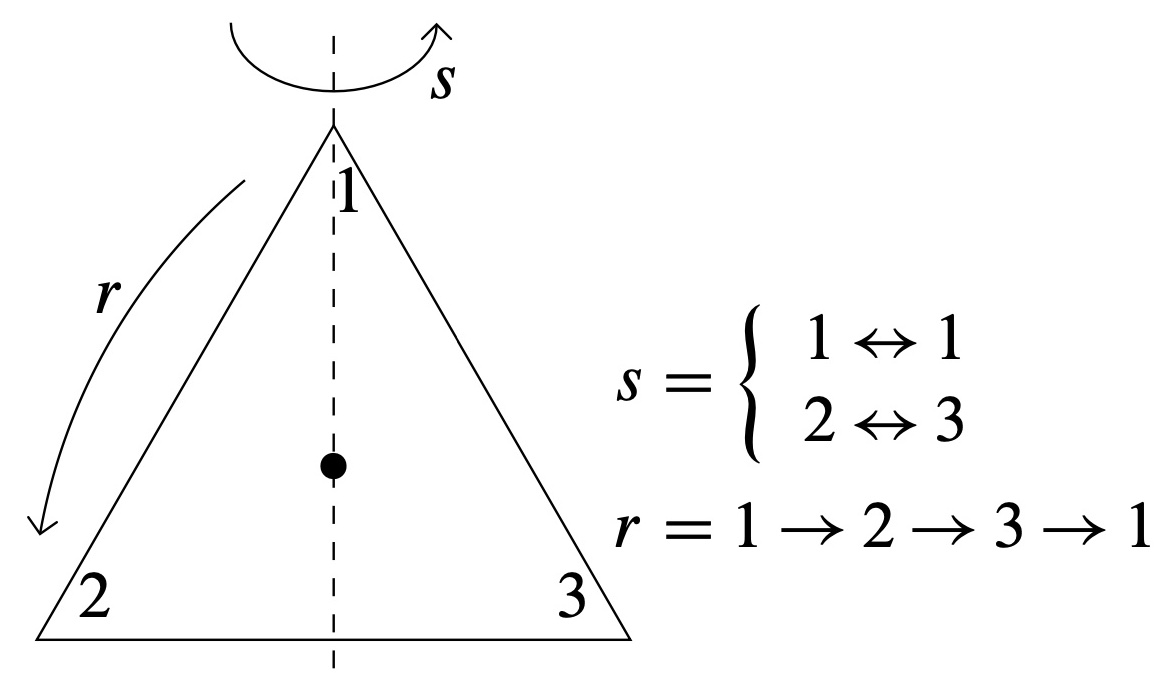
\includegraphics[width=5.5cm]{basics-of-groups/d3.jpg}}
    \caption{Symmetries of an Equilateral Triangle}
\end{figure}

What actions could we perform in order to maintain symmetry on an equilateral triangle? Well, we could rotate the triangle in $120^\circ$ anti-clockwise increments about the center of the triangle. We denote this action by the symbol $r$. Another thing we could do is reflect the triangle about the line going through one of the vertices and the center, like we discussed in an earlier chapter. This action is denoted by $s$.

Now, suppose we define $r$ to be the $120^\circ$ anti-clockwise rotation about the center and $s$ be the reflection of the triangle about the line going through vertex 1 and the center, like shown in the diagram. How do we obtain a $240^\circ$ anti-clockwise rotation? Well, we apply two $120^\circ$ anticlockwise rotations one after another. In other words, if $\ast$ means ``action composition'', then a $240^\circ$ rotation would be represented by $r^2$. Note that $r^3$, which represents a $360^\circ$ anti-clockwise rotation, is the same as doing nothing. So $r^3 = e$. Similarly, applying the reflection $s$ twice in a row (i.e., $s^2$) is the same as doing nothing, so $s^2 = e$. Thus, we have
\[
    r^3 = s^2 = e
\]
for the case of an equilateral triangle.

There's another relationship governing $r$ and $s$. Consider this: how do we obtain a reflection about the line through vertex 3 and the center? Well, we apply $r$ first, followed by $s$. This means that a reflection about the line through vertex 3 and the center is given by $rs$. Notice that this is the same thing as reflecting first and then applying $r$ twice, i.e. $sr^2$. Thus, we have the second relationship:
\[
    rs = sr^2
\]
for the case of an equilateral triangle.

The group of symmetries of an equilateral triangle is called the \textbf{dihedral group of order 6} (or the \textbf{dihedral group of degree 3}) and is denoted by $D_3$. In general,
\begin{definition}
    The \textbf{dihedral group of order $2n$}\index{dihedral group!of order $2n$} (or the \textbf{dihedral group of degree $n$}\index{dihedral group!of degree $n$}) is denoted by $D_n$ and can be thought of as the symmetries of a regular polygon of $n$ sides (a regular $n$-gon).
\end{definition}

\newpage

\begin{example}
    The symmetries of the square is given by the group $D_4$.
\end{example} 
\begin{figure}[h]
    \centering
    \fbox{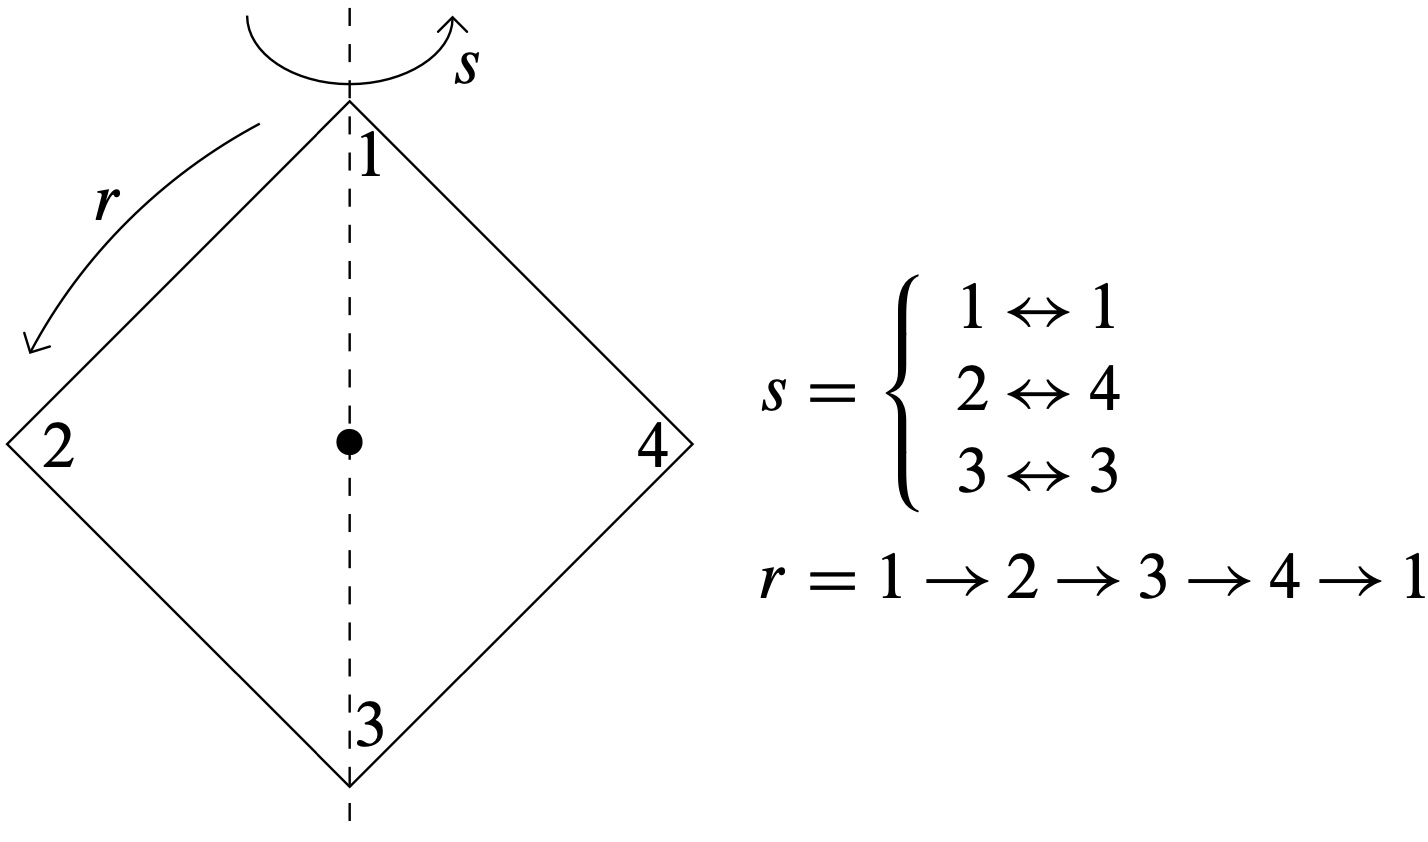
\includegraphics[width=5.5cm]{basics-of-groups/d4.jpg}}
    \caption{Symmetries of a Square}
\end{figure}

Thus, in general, the set $D_n$ consists of the following elements.
\[
    D_n = \{e, r, r^2, \dots, r^{n-1}, s, rs, r^2s, \dots, r^{n-1}s\}
\]
with the relationship between $r$ and $s$ given by $r^n = s^2 = e$ and $rs = sr^{n-1}$.

\begin{remark}
    Some authors (e.g. \cite{humphreys_1996}) will write the reflections of $D_n$ with $s$ leading $r$, i.e. $s, sr, sr^2, sr^3, \dots, sr^{n-1}$. The underlying definition, however, remains the same in either case.
\end{remark}

These relationships are succinctly given by the \textit{presentation}\index{presentation}
\[
    D_n = \langle r, s \vert r^n = s^2 = e, rs = sr^{n-1} \rangle
\]
where $r$ and $s$ can be thought of as `generators'\index{presentation!generators} and the conditions\index{presentation!conditions} are given on the right side of the pipe ($|$).

\newpage

\begin{example}\label{example-presentation-of-D3}
    The group $D_3$ has presentation
    \[
        D_3 = \langle r, s \vert r^3 = s^2 = e, rs = sr^2 \rangle.
    \]
    The Cayley table of $D_3$ is given below.

    \begin{table}[h]
        \centering
        \begin{tabular}{|l|l|l|l|l|l|l|}
        \hline
        $\boldsymbol{\ast}$ & $\boldsymbol{e}$ & $\boldsymbol{r}$ & $\boldsymbol{r^2}$ & $\boldsymbol{s}$ & $\boldsymbol{rs}$ & $\boldsymbol{r^2s}$ \\ \hline
        $\boldsymbol{e}$    & $e$    & $r$    & $r^2$  & $s$    & $rs$   & $r^2s$ \\ \hline
        $\boldsymbol{r}$    & $r$    & $r^2$  & $e$    & $rs$   & $r^2s$ & $s$    \\ \hline
        $\boldsymbol{r^2}$  & $r^2$  & $e$    & $r$    & $r^2s$ & $s$    & $rs$   \\ \hline
        $\boldsymbol{s}$    & $s$    & $r^2s$ & $rs$   & $e$    & $r^2$  & $r$    \\ \hline
        $\boldsymbol{rs}$   & $rs$   & $s$    & $r^2s$ & $r$    & $e$    & $r^2$  \\ \hline
        $\boldsymbol{r^2s}$ & $r^2s$ & $rs$   & $s$    & $r^2$  & $r$    & $e$    \\ \hline
        \end{tabular}
    \end{table}

    We use the convention of reading the \textbf{row before the column}, so the action $rs \ast r^2$ (which is usually written as $rsr^2$) is given by the row of $rs$ and the column of $r^2$, which is $r^2s$.
\end{example}

The \textit{canonical form}\index{dihedral group!canonical form} of an element in a dihedral group is $r^ms^n$, where $m$ and $n$ are non-negative integers. So how do we find the canonical form of elements like $sr$ or $srs$? We have this useful proposition to help.
\begin{proposition}
    In $D_n$, we have $r^ms = sr^{n-m}$ for all integers $1 \leq m < n$.
\end{proposition}
\begin{proof}
    We induct on $m$.
    
    When $m = 1$, $rs = sr^{n-1}$ by the definition of $D_n$.
    
    Assume now that for some integer $1 \leq k < n$, we have $r^ks = sr^{n-k}$. We consider two cases.
    \begin{itemize}
        \item If $k = n - 1$, then $k + 1 = n$. Thus, $r^{k+1}s = r^ns = s$ since $r^n = e$. Note that $sr^{(k+1)-n} = sr^{n-n} = sr^0 = s$. Therefore $r^{k+1}s = sr^{(k+1)-n}$ for the case when $k = n - 1$.
        \item The other case is if $1 \leq k \leq n - 2$. Then we have
        \begin{align*}
            r^{k+1}s &= r^k(rs)\\
            &= r^k(sr^{n-1}) & (\text{base case})\\
            &= (r^ks)r^{n-1} & (\text{associativity})\\
            &= (sr^{n-k})r^{n-1} & (\text{by induction hypothesis})\\
            &= sr^{2n - k - 1}\\
            &= sr^nr^{n-k-1}\\
            &= sr^{n-(k+1)} & (\text{since } r^n = e)
        \end{align*}
        which means $r^{k+1}s = sr^{n-(k+1)}$.
    \end{itemize}
    In either case, the statement is true for $k+1$.
    
    Therefore $r^ms = sr^{n-m}$ for all integers $1 \leq m < n$.
\end{proof}

\begin{exercise}
    Simplify $rsr^4sr^3$ in the group $D_6$.
\end{exercise}

\newpage

\section{Problems}
\begin{problem}
    Draw the Cayley table for $D_4$, the dihedral group of order 8, representing the symmetries of a square.\newline
    By referring to the Cayley table,
    \begin{partquestions}{\alph*}
        \item explain why $D_4$ is \textbf{not} abelian;
        \item simplify $r^3srsr^3sr^3sr^2$.
    \end{partquestions}
\end{problem}

\begin{problem}
    Let $G$ be a group. If every element in $G$ is its own inverse, show that $G$ is abelian.
\end{problem}

\begin{problem}\label{problem-element-to-power-of-multiple-of-order-is-identity}
    Let $G$ be a group with identity $e$. Suppose an element $x$ in $G$ has finite order $n$. Prove that a positive integer $m$ is a multiple of $n$ if and only if $x^m = e$.\newline
    (\textit{Hint: consider Euclid's division lemma (\myref{lemma-euclid-division}) to prove one direction of the claim.})
\end{problem}

\begin{problem}
    Let $G$ be a group.
    \begin{partquestions}{\alph*}
        \item Suppose $(gh)^2 = g^2h^2$ for all elements $g$ and $h$ in $G$. Prove that $G$ is abelian.
        \item Suppose $G$ is abelian. Prove that $(gh)^n = g^nh^n$ for all elements $g$ and $h$ in $G$ and for all positive integers $n$.
    \end{partquestions}
\end{problem}

\begin{problem}
    Let $G = (\mathbb{Z}_n, \oplus_n)$. It is given $G$ is a group. Show that $G$ is a cyclic group of order $n$.
\end{problem}

\newpage

\begin{problem}
    Let the set $S = \mathbb{R}^2$, that is,
    \[
        S = \{(x, y) \vert x, y \in \mathbb{R}\}.
    \]
    Let the transformation $T: S \to S$ is defined by
    \[
        T(x, y) = (-y, x+y).
    \]
    Define the set $A = \{T^r \vert r \in \mathbb{Z} \text{ and } r \geq 1\}$. Show that $A$ is a group under function composition ($\circ$), and state the order of this group.
\end{problem}
